% Slide bảo vệ giữa kỳ, phần A (Bùi Thuỳ Châu Anh).
% Biên dịch bằng XeLaTeX (Overleaf: Menu > Compiler > XeLaTeX).
\documentclass[aspectratio=169,11pt]{beamer}

\usepackage{fontspec}
\setmainfont{texgyreheros}[Extension=.otf,UprightFont=*-regular,BoldFont=*-bold,ItalicFont=*-italic,BoldItalicFont=*-bolditalic]
\setsansfont{texgyreheros}[Extension=.otf,UprightFont=*-regular,BoldFont=*-bold,ItalicFont=*-italic,BoldItalicFont=*-bolditalic]
\setmonofont{texgyrecursor}[Extension=.otf,UprightFont=*-regular,BoldFont=*-bold,ItalicFont=*-italic,BoldItalicFont=*-bolditalic]
\usepackage[vietnamese]{babel}
\usepackage{tikz}
\usetikzlibrary{arrows.meta,positioning,calc}
\usepackage{tabularx}
\usepackage{booktabs}
\usepackage{colortbl}
\usepackage{array}

% ---- Màu: xanh tableheader của báo cáo làm màu nhấn ----
\definecolor{accent}{RGB}{68,114,196}
\definecolor{accentlight}{RGB}{234,240,250}
\definecolor{accentdark}{RGB}{38,62,110}
\definecolor{ink}{RGB}{38,42,52}
\definecolor{muted}{RGB}{110,116,128}
\definecolor{warn}{RGB}{196,80,90}

\setbeamercolor{normal text}{fg=ink,bg=white}
\setbeamercolor{structure}{fg=accent}
\setbeamercolor{frametitle}{fg=accentdark,bg=white}
\setbeamercolor{itemize item}{fg=accent}
\setbeamercolor{itemize subitem}{fg=accent}
\setbeamercolor{block title}{fg=white,bg=accent}
\setbeamercolor{block body}{fg=ink,bg=accentlight}
\setbeamertemplate{navigation symbols}{}
\setbeamertemplate{itemize item}[square]
\setbeamertemplate{itemize subitem}[circle]
\setbeamerfont{itemize/enumerate body}{size=\normalsize}
\setbeamerfont{itemize/enumerate subbody}{size=\small}
\setbeamertemplate{blocks}[rounded][shadow=false]

% Tiêu đề khung: chữ đậm xanh đậm + vạch xanh
\setbeamertemplate{frametitle}{%
  \vskip 3mm
  \usebeamercolor[fg]{frametitle}\usebeamerfont{frametitle}\bfseries\Large\insertframetitle\par
  \vskip 1.2mm
  {\color{accent}\hrule height 1.2pt}
}
% Chân trang: tên + số trang
\setbeamertemplate{footline}{%
  \hbox to \paperwidth{%
    \hspace{8mm}\color{muted}\scriptsize Bùi Thuỳ Châu Anh \textbar\ Phát hiện biển số xe và tách ký tự bằng xử lý ảnh cổ điển%
    \hfill\insertframenumber\,/\,\inserttotalframenumber\hspace{8mm}}
  \vskip 4mm}
\setbeamersize{text margin left=9mm,text margin right=9mm}

\newcommand{\code}[1]{{\footnotesize\ttfamily #1}}
\newcommand{\acc}[1]{\textcolor{accent}{\textbf{#1}}}
\newcommand{\hl}[1]{\textcolor{accentdark}{\textbf{#1}}}

\renewcommand{\arraystretch}{1.18}
\newcommand{\barrow}[4]{%
  \node[anchor=east,align=right] at (-1.5,#1) {#2};
  \fill[accent] (0,#1-0.26) rectangle (#3,#1+0.26);
  \node[anchor=west] at (#3+1.5,#1) {#4};}
\newcommand{\hd}[1]{\cellcolor{accent}\textcolor{white}{\bfseries #1}}
\newcolumntype{C}{>{\centering\arraybackslash}X}
\newcolumntype{Y}{>{\raggedright\arraybackslash}X}

\title{Phát hiện biển số xe và tách ký tự\\bằng xử lý ảnh cổ điển}
\subtitle{Báo cáo giữa kỳ, phần A: tiền xử lý, định vị, nắn phối cảnh, phân tích lỗi}
\author{Bùi Thuỳ Châu Anh (24001963)\and Nguyễn Ngọc Bích (24001977)}
\date{MAT3562E Computer Vision, HK1 2026--2027}

\begin{document}

% ============ 1. Tiêu đề ============
\begin{frame}[plain]
  \begin{tikzpicture}[remember picture,overlay]
    \fill[accent] (current page.north west) rectangle ([yshift=-4.2cm]current page.north east);
    \node[anchor=north west,xshift=9mm,yshift=-7mm,text=white,align=left] at (current page.north west)
      {\fontsize{9}{11}\selectfont\bfseries ĐẠI HỌC KHOA HỌC TỰ NHIÊN, ĐHQGHN};
    \node[anchor=north east,xshift=-9mm,yshift=-5mm,fill=white,rounded corners=3pt,inner sep=2.5mm] at (current page.north east)
      {
\includegraphics[height=2.3cm]{figures/HUS.png}};
    \node[anchor=south west,xshift=9mm,yshift=-4.2cm+4mm,text=white,align=left,text width=0.72\paperwidth] at (current page.north west)
      {\fontsize{22}{26}\selectfont\bfseries Phát hiện biển số xe và tách ký tự bằng xử lý ảnh cổ điển};
  \end{tikzpicture}
  \vspace{3.55cm}
  \begin{flushleft}
    {\large\bfseries\color{accentdark} Báo cáo giữa kỳ: phần A}\\[1mm]
    {\color{muted}Tiền xử lý, định vị biển, nắn phối cảnh và phân tích lỗi}\\[5mm]
    \small
    \begin{tabular}{@{}l@{\hspace{6mm}}l@{}}
      \hl{Nhóm thực hiện} & Bùi Thuỳ Châu Anh (24001963), Nguyễn Ngọc Bích (24001977)\\
      \hl{Môn học} & MAT3562E Computer Vision, HK1 2026--2027\\
      \hl{Giảng viên} & TS. Cao Văn Chung\\
    \end{tabular}
  \end{flushleft}
\end{frame}

% ============ 2. Bài toán + dữ liệu ============
\begin{frame}{Bài toán và dữ liệu}
  \begin{columns}[T]
    \column{0.50\textwidth}
    \begin{itemize}
      \item Kịch bản: camera cố định ở bãi gửi xe, mỗi ảnh có đúng một biển.
      \item Đầu ra giữa kỳ: hộp biển, ảnh biển đã nắn, danh sách hộp ký tự.
      \item Chỉ dùng \hl{xử lý ảnh cổ điển}, không học sâu.
      \item Dữ liệu: tập con CCPD2019, 660 ảnh biển xanh 7 ký tự: \code{base} 500 và bốn nhóm khó (\code{tilt}, \code{blur}, \code{db}, \code{challenge}) mỗi nhóm 40.
      \item Chọn tham số trên \acc{tune} (30\%), chỉ báo cáo trên \acc{test} (70\%).
    \end{itemize}
    \column{0.48\textwidth}
    \vspace{2mm}
    \small
    \begin{tabularx}{\linewidth}{>{\raggedright\arraybackslash}Xrr}
      \rowcolor{accent}\hd{Nhóm} & \hd{tune} & \hd{test}\\
      base & 150 & 350\\
      \rowcolor{accentlight}mỗi nhóm khó & 12 & 28\\
      \textbf{Tổng} & \textbf{198} & \textbf{462}\\
    \end{tabularx}
    \vspace{4mm}

    \begin{block}{Độ đo}
      \small
      IoU $\ge 0.5$ với bbox thật; P, R, F1 theo top-1; Recall@$k$ (R@5 là trần của bước xếp hạng).
    \end{block}
  \end{columns}
\end{frame}

% ============ 3. Pipeline ============
\begin{frame}{Pipeline và phân công}
  \centering
  \vspace{1mm}
  \begin{tikzpicture}[
    node distance=8mm and 5mm,
    boxA/.style={draw=accent,fill=accentlight,thick,rounded corners=3pt,align=center,minimum height=19mm,text width=27mm,font=\footnotesize},
    boxB/.style={draw=muted,dashed,thick,rounded corners=3pt,align=center,minimum height=19mm,text width=27mm,font=\footnotesize,text=muted},
    arr/.style={-{Stealth[length=2.4mm]},thick,color=accentdark}]
    \node[boxA] (in) {Ảnh xe (BGR)};
    \node[boxA,right=of in] (pre) {\textbf{Tiền xử lý}\\resize 800, xám,\\CLAHE, lọc nhiễu};
    \node[boxA,right=of pre] (edge) {\textbf{Định vị theo cạnh}\\Sobel-x, Otsu,\\morph đa tỉ lệ,\\lọc, NMS};
    \node[boxA,right=of edge] (svm) {\textbf{HOG + SVM}\\xếp lại top-5\\(biến thể A+SVM)};
    \node[boxA,below=of svm] (top1) {Chọn top-1\\(bbox + quad)};
    \node[boxA,left=of top1] (quad) {\textbf{Ước lượng quad}\\từ mặt nạ xanh\\(HSV)};
    \node[boxA,left=of quad] (warp) {\textbf{Nắn phối cảnh}\\homography về\\ảnh $220\times 70$};
    \node[boxB,left=of warp] (partb) {\textbf{Phần B (Bích)}\\nhị phân hóa,\\tách ký tự};
    \draw[arr] (in)--(pre); \draw[arr] (pre)--(edge); \draw[arr] (edge)--(svm);
    \draw[arr] (svm)--(top1); \draw[arr] (top1)--(quad); \draw[arr] (quad)--(warp); \draw[arr] (warp)--(partb);
    \node[boxA,minimum height=4mm,text width=4mm,inner sep=0pt,below=7mm of partb.south west,anchor=north west] (la) {};
    \node[right=2mm of la,font=\small] {Phần A (Châu Anh): ba bước đầu và đánh giá};
    \node[boxB,minimum height=4mm,text width=4mm,inner sep=0pt,below=3mm of la.south west,anchor=north west] (lb) {};
    \node[right=2mm of lb,font=\small] {Phần B (Bích): hệ màu, nhị phân hóa, tách ký tự};
  \end{tikzpicture}
\end{frame}

% ============ 4. Tiền xử lý + E2 ============
\begin{frame}{Tiền xử lý và thí nghiệm E2: bộ lọc nhiễu}
  \begin{columns}[T]
    \column{0.42\textwidth}
    \begin{itemize}
      \item Resize về rộng \acc{800} px (ảnh lớn hơn thì tốt hơn), ảnh xám.
      \item CLAHE (clip 2.0, lưới $8\times8$) cân bằng sáng cục bộ.
      \item So sánh 4 bộ lọc: \code{none}, \code{gaussian}, \code{median}, \code{bilateral}.
      \item Chọn \hl{bilateral} theo F1 trên tune (0.761 so với 0.584--0.624).
      \item Giá phải trả: chậm hơn khoảng 18--29 ms/ảnh.
    \end{itemize}
    \column{0.56\textwidth}
    {\small\bfseries Tập test, $n=462$, \code{localize\_edge}}\\[1mm]
    \small
    \begin{tabularx}{\linewidth}{lCCCC}
      \rowcolor{accent}\hd{Bộ lọc} & \hd{F1} & \hd{R@1} & \hd{R@5} & \hd{ms/ảnh}\\
      \rowcolor{accentlight}\textbf{bilateral} & \textbf{0.705} & \textbf{0.682} & \textbf{0.792} & 111.1\\
      gaussian & 0.630 & 0.615 & 0.712 & 82.4\\
      \rowcolor{accentlight}median & 0.600 & 0.584 & 0.699 & 93.2\\
      none & 0.592 & 0.576 & 0.645 & 84.7\\
    \end{tabularx}
    \vspace{2mm}

    {\footnotesize\color{muted} Lý do bilateral tốt hơn (giữ cạnh nét chữ, giảm ứng viên rác) mới là giả thuyết, chưa kiểm tra riêng. Thời gian chỉ so tương đối.}
  \end{columns}
\end{frame}

% ============ 5. Định vị dựa biên + Issue 10 ============
\begin{frame}{Định vị dựa trên cạnh và Issue \#10}
  \begin{columns}[T]
    \column{0.50\textwidth}
    \begin{enumerate}
      \item $|G_x|$ Sobel theo $x$, nhị phân Otsu.
      \item \emph{Close} ngang $21\times5$ nối nét ký tự, \emph{open} $3\times3$.
      \item \hl{Đa tỉ lệ}: thêm kernel $13\times3$ và $33\times7$, gộp bằng \hl{NMS} (IoU 0.5).
      \item Lọc theo \code{aspect}, \code{area\_ratio}, \code{fill\_ratio}, \code{edge\_density}, góc.
      \item Điểm heuristic, giữ top-5.
    \end{enumerate}
    \vspace{1mm}
    {\small \textbf{Issue \#10}: nút thắt ở bộ lọc (tăng $k$ lên 10 không đổi). Sửa: hai kernel phụ, \code{area\_ratio} $[0.008,0.16]$, \code{aspect} $[1.5,7]$, chọn trên tune.}
    \column{0.48\textwidth}
    {\small\bfseries Trước và sau, tập test (\code{localize\_edge})}\\[1mm]
    \begin{tabularx}{\linewidth}{lCC}
      \rowcolor{accent}\hd{ALL ($n=462$)} & \hd{Cũ} & \hd{Chốt}\\
      Recall ứng viên (R@5) & 0.667 & \acc{0.792}\\
      \rowcolor{accentlight}Recall@1 (top-1) & 0.545 & \acc{0.682}\\
      Precision & 0.593 & \acc{0.729}\\
      \rowcolor{accentlight}Recall@1, nhóm \code{base} & 0.609 & \acc{0.751}\\
    \end{tabularx}
    \vspace{2mm}

    {\footnotesize Nhóm \code{db}, \code{challenge} gần như không đổi. Cái giá: thời gian tăng 40--50\% (đo khi máy tải, chỉ tương đối).}
  \end{columns}
\end{frame}

% ============ 6. HOG + SVM + E3 ============
\begin{frame}{Xếp hạng lại bằng HOG + SVM (E3)}
  \begin{columns}[T]
    \column{0.33\textwidth}
    \begin{itemize}
      \item Crop bbox, resize $128\times32$, HOG 1620 chiều.
      \item \code{LinearSVC}, chỉ huấn luyện trên tune (198 dương, 594 âm).
      \item Chỉ xếp lại top-5, không thêm ứng viên.
      \item Top-1 test: \hl{0.682 $\to$ 0.751} (+32 ảnh).
      \item R@5 vẫn \hl{0.792}: trần xếp hạng.
    \end{itemize}
    \column{0.65\textwidth}
    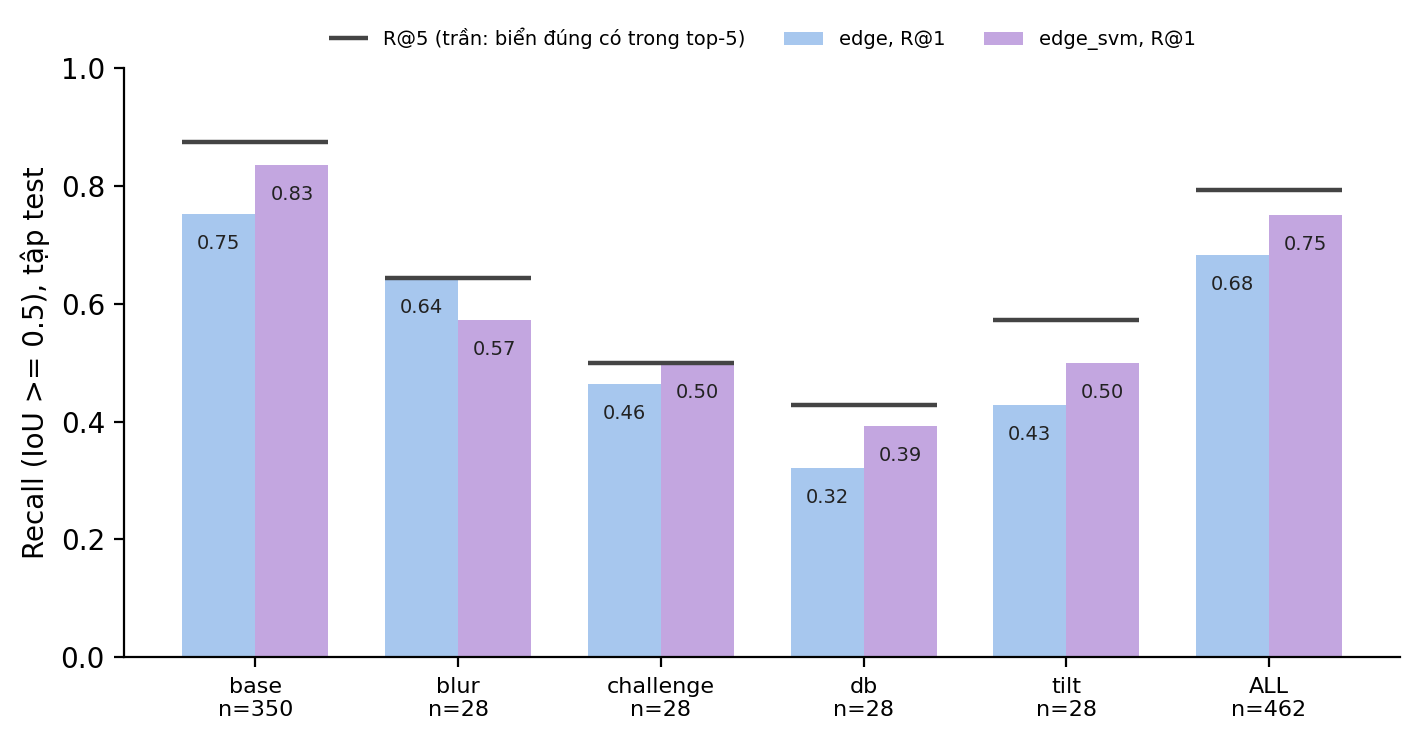
\includegraphics[width=\linewidth]{figures/e3_subset_r1.png}\\[-1mm]
    {\footnotesize\color{muted} Recall@1 theo nhóm (test), vạch đen là R@5. 21\% ảnh test không có ứng viên đúng trong top-5.}
  \end{columns}
\end{frame}

% ============ 7. Nắn phối cảnh + E4 ============
\begin{frame}{Nắn phối cảnh và thí nghiệm E4: cắt bbox hay warp quad}
  \begin{columns}[T]
    \column{0.42\textwidth}
    \begin{itemize}
      \item Quad: mặt nạ xanh HSV + \code{approxPolyDP} (mặc định), lùi về \code{minAreaRect}.
      \item Homography đưa biển về $220\times70$.
      \item Đối chứng: cắt bbox ngang rồi resize.
      \item \code{tilt}: bbox không bù được nghiêng, \code{count\_match} 0.000 so với 0.429.
    \end{itemize}
    \column{0.56\textwidth}
    {\small\bfseries Tập test, toàn pipeline}\\[1mm]
    \small
    \begin{tabularx}{\linewidth}{lCC}
      \rowcolor{accent}\hd{Chỉ số} & \hd{bbox} & \hd{Quad}\\
      Sai số góc, tb (px) & 25.2 & \acc{16.3}\\
      \rowcolor{accentlight}Sai số góc, trung vị (px) & 19.4 & \acc{13.8}\\
      \code{all\_correct}, crop \code{gt} & 0.262 & \acc{0.563}\\
      \rowcolor{accentlight}\code{all\_correct}, top-1 đúng & 0.124 & \acc{0.259}\\
      Sai số góc \code{tilt} (px) & 68.0 & \acc{28.9}\\
    \end{tabularx}
    \vspace{2mm}

    {\footnotesize\color{muted} \code{blur} là ngoại lệ (16 ảnh, chênh 1--2 ảnh, chưa kết luận). \code{approxpoly} so với \code{minarearect}: khác biệt nhỏ, $p=0.46$.}
  \end{columns}
\end{frame}

% ============ 8. E7 thời gian ============
\begin{frame}{Thời gian chạy từng bước (E7)}
  \begin{columns}[T]
    \column{0.58\textwidth}
    {\small\bfseries ms/ảnh, trung bình, tập test, một tiến trình}\\[2mm]
    \begin{tikzpicture}[xshift=9mm,x=0.050cm,y=0.9cm,font=\small]
      \barrow{3.0}{Tiền xử lý}{69.79}{69.8}
      \barrow{2.0}{Sobel, morph, lọc, NMS}{63.50}{63.5}
      \barrow{1.0}{HOG + SVM}{4.77}{4.8}
      \barrow{0.0}{Nắn, nhị phân, tách}{1.84}{1.8}
    \end{tikzpicture}
    \column{0.40\textwidth}
    \begin{itemize}
      \item Tổng \hl{139.8 ms/ảnh} (p95 262.2 ms).
      \item Định vị chiếm gần hết: tiền xử lý $\approx$ 50\% (chủ yếu bilateral), Sobel + morph $\approx$ 45\%, SVM $\approx$ 3\%.
      \item Nắn, nhị phân hóa, tách ký tự cộng lại chỉ 1.8 ms.
    \end{itemize}
  \end{columns}
  \vspace{1mm}
  \begin{block}{Lưu ý khi đọc số}
    \small Đo trên máy ít tải nhưng không phải máy chuyên dụng; lần ghi trong sổ thí nghiệm là 416 ms/ảnh (máy đang chạy nhiều tiến trình). Chỉ nên đọc tỉ lệ tương đối giữa các bước.
  \end{block}
\end{frame}

% ============ 9. Triage ============
\begin{frame}{Triage lỗi: mỗi ảnh test mất ở bước nào?}
  \begin{columns}[T]
    \column{0.62\textwidth}
    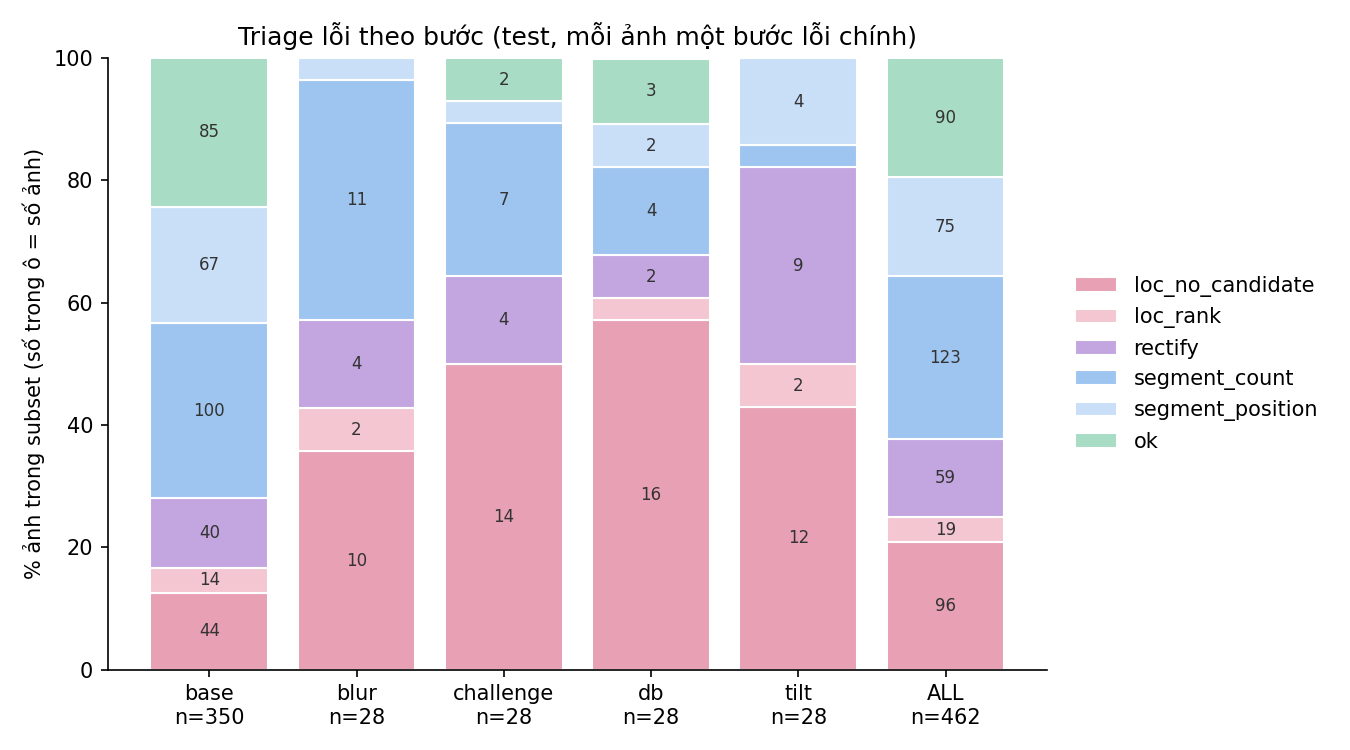
\includegraphics[width=\linewidth]{figures/triage_stages.png}
    \column{0.36\textwidth}
    \footnotesize
    \begin{tabularx}{\linewidth}{>{\raggedright\arraybackslash}Xrr}
      \rowcolor{accent}\hd{Bước lỗi chính} & \hd{Ảnh} & \hd{\%\,}\\
      \code{loc\_no\_candidate} & 96 & 20.8\\
      \rowcolor{accentlight}\code{loc\_rank} & 19 & 4.1\\
      \code{rectify} & 59 & 12.8\\
      \rowcolor{accentlight}\code{segment\_count} & 123 & 26.6\\
      \code{segment\_position} & 75 & 16.2\\
      \rowcolor{accentlight}\code{ok} & \textbf{90} & \textbf{19.5}\\
    \end{tabularx}
    \vspace{2mm}

    {\footnotesize Mỗi ảnh một bước lỗi chính, xét theo thứ tự pipeline. Nhóm khó gần như không có ảnh \code{ok} (0--3 trên 28).}
  \end{columns}
\end{frame}

% ============ 10. Phát hiện chính ============
\begin{frame}{Phát hiện chính từ phân tích lỗi}
  \begin{columns}[T]
    \column{0.62\textwidth}
    \begin{itemize}
      \item \hl{Định vị mất ở khâu sinh ứng viên}: 96 ảnh \code{loc\_no\_candidate} so với 19 ảnh \code{loc\_rank}; chỉ 12/96 do bbox nhỏ hơn cận diện tích.
      \item \hl{Xếp hạng}: 18/19 ảnh có biển đúng ở hạng 2; top-1 thường là logo hoặc chữ hãng xe.
      \item \hl{Crop dự đoán và bộ tách cùng bậc}: trong 257 ảnh top-1 đúng nhưng vẫn lỗi, \acc{152} tách đúng ở crop \code{gt} (lỗi do crop dự đoán), \acc{105} tách sai cả ở crop \code{gt} (lỗi do bộ tách).
      \item 54/123 ảnh \code{segment\_count} có 6 hộp do ký tự Hán dính chữ A (phần của B).
    \end{itemize}
    \column{0.34\textwidth}
    \centering
    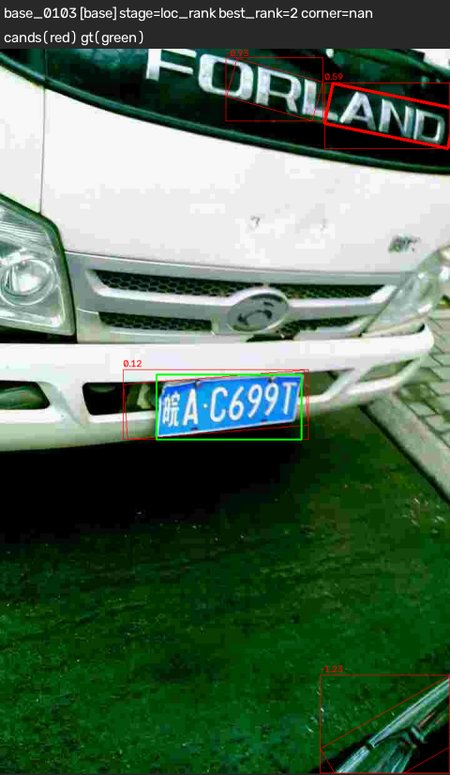
\includegraphics[height=0.58\textheight]{figures/loc_rank_cands.png}\\[-1mm]
    {\footnotesize\color{muted} \code{loc\_rank}: ứng viên đỏ, bbox thật xanh. Top-1 là chữ hãng xe, biển thật ở hạng 2.}
  \end{columns}
\end{frame}

% ============ 11. Hạn chế + hướng ============
\begin{frame}{Hạn chế và hướng cải thiện}
  \begin{columns}[T]
    \column{0.50\textwidth}
    {\bfseries\color{accentdark}Hạn chế}
    \begin{itemize}
      \item IoU trục ngang phạt biển nghiêng.
      \item Nhóm khó chỉ 28 ảnh test (một ảnh = 0.036), chưa có khoảng tin cậy, một lần chia tune/test.
      \item CV của SVM chia theo patch nên lạc quan.
      \item Chọn \code{approxpoly} dựa trên 128 ảnh tune, ngưỡng triage trên 50 ảnh.
      \item Thời gian đo trên máy không chuyên dụng.
    \end{itemize}
    \column{0.48\textwidth}
    {\bfseries\color{accentdark}Hướng cải thiện}
    \begin{itemize}
      \item Thêm nguồn ứng viên theo \hl{màu biển} hoặc bù nghiêng trước morph (chưa thử); 21\% ảnh không có ứng viên đúng.
      \item SVM: thêm \hl{mẫu âm khó} (logo, chữ hãng xe), chia fold theo ảnh.
      \item Nắn: quad chính xác hơn (sai số $\approx$ 16 px).
      \item Đánh giá bằng \hl{IoU đa giác}.
    \end{itemize}
  \end{columns}
\end{frame}

% ============ 12. Phần của Bích ============
\begin{frame}{Phần của Bích}
  \centering
  \vspace{8mm}
  {\Large\bfseries\color{accentdark} Nguyễn Ngọc Bích (24001977)}\\[4mm]
  {\color{muted}Hệ màu, nhị phân hóa, tách ký tự}\\[8mm]
  \begin{tabular}{@{}ll@{}}
    \acc{E1} & phân tích hệ màu\\
    \acc{E5} & nhị phân hóa: Otsu và adaptive\\
    \acc{E6} & tách ký tự: CCA và projection\\
    \acc{E8} & ảnh biển số Việt Nam tự chụp, đánh giá định tính\\
  \end{tabular}
  \vfill
  {\footnotesize\color{muted}Nội dung và số liệu do Bích trình bày.}
\end{frame}

% ============ 13. Cảm ơn ============
\begin{frame}[plain]
  \begin{tikzpicture}[remember picture,overlay]
    \fill[accent] (current page.south west) rectangle (current page.north east);
    \node[text=white,align=center,text width=0.8\paperwidth] at (current page.center)
      {{\fontsize{28}{32}\selectfont\bfseries Cảm ơn thầy và các bạn đã lắng nghe}\\[6mm]
       {\large Xin mời thầy và các bạn đặt câu hỏi}};
  \end{tikzpicture}
\end{frame}

\end{document}
